% !TEX root = ../Dokumentation.tex
\subsection{Intelligente Systeme}

\subsubsection{Software auf Mini-Computer}
Das Softwarekonzept basiert auf dem MVC\footnote{MVC = Model-View-Control}-Prinzip, wobei sich die View auf einen reinen Debug-Zweck beschränkt. Der Controller kommunziert mit allen Subprozesse und grenzt an die Schnittstelle zur Hardwaresteuerung. Um die Performance des Rasperry Pi möglichst auszunutzen wird mit Threads gearbeitet. Die parallel laufenden Subprozesse sind:

\begin{itemize}
\item Bilderzeugung,
\item Objekterkennung und
\item Fahrbahnerkennung.
\end{itemize}

\begin{figure}[H]
	\centering
	\includegraphics[width=0.8\textwidth]{03_Loesungskonzept/pictures/grobablauf.png}
	\caption{Aktivitätendiagramm Grobablauf}
\end{figure}

Der Zustand des Fahrzeuges wird im Model gespeichert und steht allen Prozessen zur Verfügung. Die Datenstruktur ist dabei so aufgebaut, dass keine Zugriffskonflikte entstehen sollten.\\
Der Controller behandelt alle Anweisungen der Prozesse. Meldet beispielsweise die Objekterkennung einen Container, hat dieser Priorität vor dem normalen Fahren und das Mikrocontroller-Board erhält die entsprechenden Anweisungen. Das folgende Diagramm zeigt eine Gesamtübersicht von den verschiedenen Komponenten.\\[0.2cm]
\begin{figure}[H]
\centering
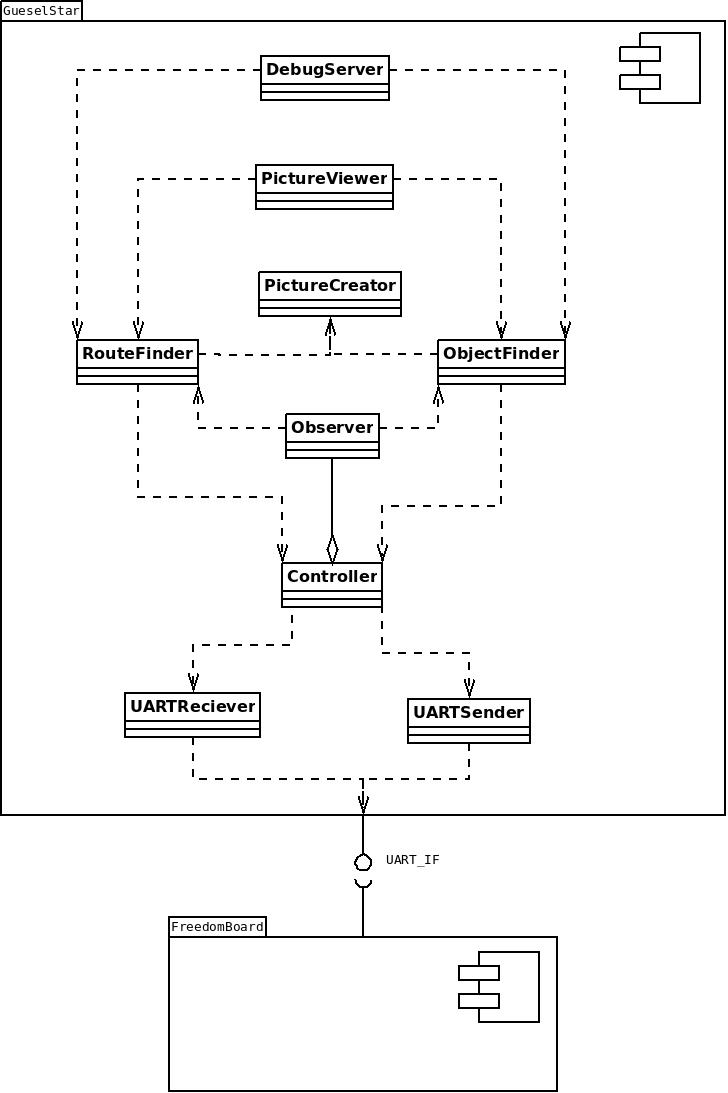
\includegraphics[width=0.8\textwidth]{03_Loesungskonzept/pictures/Komponentendiagramm_detailliert_v2.jpeg}
\caption{Komponentendiagramm}
\end{figure}

\textbf{Debug-View}\\[0.2cm]
Um während der Implementierungs-Phase der geschriebene Code zu testen wurde eine Debug-View entwickelt. Mit dieser kann auf den Debug-Server, welcher auf dem Raspberry Pi gestartet wird, zugegriffen werden. Nach einer erfolgreichen Verbindung werden die aufgenommenen Bilder vom Server an den Client (GueselStarObserver) gesendet.

\begin{figure}[H]
\centering
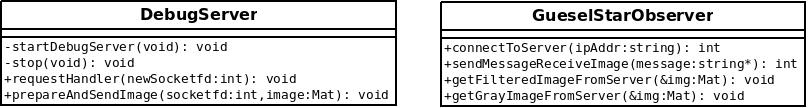
\includegraphics[width=0.8\textwidth]{03_Loesungskonzept/pictures/DebugView.jpeg}
\caption{Debug-View}
\end{figure}

Die Kommunikation zwischen Server und Client läuft über TCP/IP. Auf dem Server wird ein Server-Socket geöffnet, auf welches sich der Client verbinden kann.

\textbf{Konfiguration}\\[0.2cm]
Neu geschriebener Code benötigt einen erneuten Build. Um einen neuen Build, welcher Zeit benötigt, zu unterbinden wurde eine Konfigurations-Datei erstellt, in welcher alle benötigten Parameter angepasst werden können. Das Einlesen der Konfiguration erfolgt über einen selbstentwickelten Parser und wird anschliessend in einem Objekt der Klasse "PRENConfiguration" abgespeichert.

\begin{figure}[H]
\centering
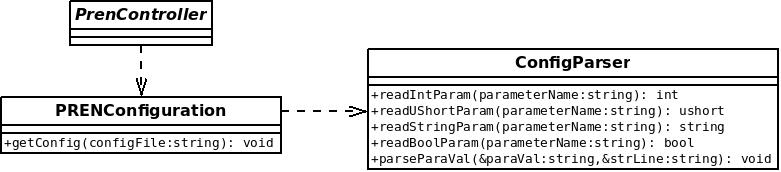
\includegraphics[width=0.8\textwidth]{03_Loesungskonzept/pictures/Configuration.jpeg}
\caption{Konfiguration}
\end{figure}
 
%***************************
\subsubsection{Software auf Mikrocontrollerboard}


\textbf{SW Architektur}\\[0.2cm]
Auf dem Mikrocontroller (Freedomboard KL25Z) wurde mit dem Betriebssystem FreeRTOS gearbeitet. Dies ermöglicht die Erstellung von verschiedenen Tasks. Dies erlaubt eine bessere Trennung der einzelnen Softwarekomponenten und erleichtert das Programmieren. Die verschiedenen Tasks wurden bereits im PREN1 geplant und nun im PREN2 umgesetzt. 
Hier eine Übersicht der Tasks und Events:

\begin{figure}[H]
	\centering
	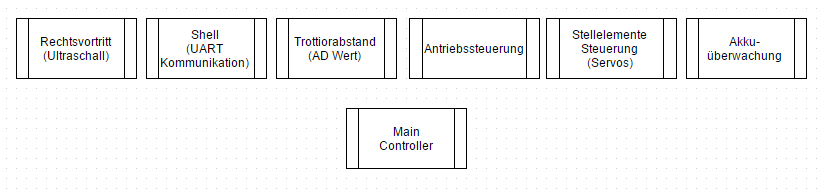
\includegraphics[width=0.9\textwidth]{03_Loesungskonzept/pictures/MC_Tasks.png}
	\caption{Übersicht MC Tasks}
\end{figure}
In den folgenden Abschnitten werden kurz auf die einzelnen Tasks und Events eingegangen. Dies dient jedoch nur der Übersicht.\\
\textbf{Controller}\\[0.2cm]
Dieser Task steuert das Freedomboard. Das heisst konkret, dass dieser Task das initialisieren, fahren, aufladen, entladen  und beenden des Programmes zuständg ist. Dies ist über eine FineState Maschiene realisiert, welche bei besonderen Events den State wechselt. Ein besonderer Event ist zum Beispiel das Startkommando über die Kommunikation oder eine Unterspannung am Akku.\\[0.2cm]
\textbf{Kommunikation}\\[0.2cm]
Dieser Task übernimmt die Auswertung der erhaltenen Kommandos über die UART Schnittstelle. Dies geschieht über eine sogenannte Parsertabelle. In dieser Parsertabelle können beliebig weitere Kommandos (Funktionen) hinzugefügt werden. Dieser Task wird alle 10ms aufgerufen, da die Kommunikation mit dem Raspberry Pi möglichst schnell funktionieren soll.\\[0.2cm]
\textbf{Analog-Digitalwandlung}\\[0.2cm]
Dieser Task holt und verarbeitet die Daten aus dem Analog Digitalwandler des KL25Z. Das heisst konkret es werden beide Akku Spannungen ausgelesen und überwacht. Zudem wird der Widerstandswert des Flexsensensors eingelesen und damit der Abstand zum Gehsteig berechnet. Zur Akkuüberwachung folgen weiter im Text weitere Informationen.\\[0.2cm]
\textbf{Geschwindigkeitsregelung}\\[0.2cm]
Der Geschwindigkeitsregelungstask regelt die Geschwindigkeit des DC-Antriebmotors. Dies geschieht über einen PID Regler. Dieser wurde vom Modul Mikrocontrollertechnik an der Hochschule Luzern übernommen und nach den eigenen Bedürfnissen angepasst. Wie die PID Werte berechnet wurden und der Regelkreis aussieht wird noch separat erläutert.\\[0.2cm]
\textbf{Ultraschall}\\[0.2cm]
Dieser Task steuert den Ultraschallsensor an. Dies wurde nach einem Tutorial von mcuoneclipse.com realisiert und auf die Softwareumgebung noch weiter angepasst.\\[0.2cm]
\textbf{Master check}\\[0.2cm]
Dieser Task ist die Lebensversicherung des Fahrzeugs. Hier wird überprüft ob der Master (Raspberry Pi) noch angeschlossen und Funktionstüchtig ist. Wenn das Mikrocontrollerborad nicht innerhalb von wenigen Sekunden eine Bestätigungsmeldung des Masters bekommt, wird das Freedomboard in den Beendet Modus wechseln und fährt somit nicht unkontrolliert herum. \\[0.2cm]
\textbf{Event}\\[0.2cm]
Die Events treten unregelmäßig und ungeplant auf. Diese unterbrechen das normale Programm (Interrupt) und führen einen eigenen kurzen Programmcode aus. Dies ist bei den im Bild aufgeführten Funktionen der Fall.\\[0.2cm]
\textbf{Akkuüberwachung Schwellwertberechnung}\\[0.2cm]
Damit die LiPo-Akkumulatoren nicht zerstört werden, muss sichergestellt werden das diese nicht tief entladen werden. Dies wird über das Freedomboard gelöst. Die Akkuspannung wird über einen Analog - Digitalwandler eingelesen. Wenn die Akkuspannung einen gewissen Wert unterschreiten, werden die Verbraucher an den Akkus "abgeschaltet". Eine Lipozelle sollte die Zellenspannung von 3.5V nicht unterschreiten. Im Normalfall sollten alle Zellen einzeln überwacht werden, dies ist jedoch im Rahmen dieses Prototypen nicht angemessen. Als Kompromiss wird gesamte Ausgangsspannung gemessen. Das heisst zwei beziehungsweise drei Zellen in Serie (je nach Akku). Als Abschaltwert für eine Zelle wurde 3.7V bestimmt.\\
Das Freedomboard kann nur Spannungen bis 3.3V einlesen. Daher ist ein Spannungsteiler nötig. Damit dieser Wert sicher nicht überschritten wird, wird mit einer maximal zulässigen Spannung von 3V gerechnet. Für UAkku wurde 13V gewählt, damit der AD-Wandler sicher nie 3V erreicht.\\
Für den zweiten Akku (11.1V):
\[	U_Akku/U_Frd=R1/R2\]
\[	13V/3V=4.33=g\]
Gewählt:
\[	R2=10k R1=R2*4.33=43kOhm\]
Der Abschaltwert des drei Zellen Akkus ist 3.7V * 3= 11.1V.
11.1V nach dem Spannungswandler entspricht einer Spannung von \[Uin/g=11.1V*10/53.3=2.075V\]
3.3V enspricht 65'535. Somit entspricht eine Spannung von 2.075V einem eingelesenen Spannungswert von 41592. Falls dieser Wert über längere (wenige Sekunden) unterschritten wird, wird eine Nachricht an das Raspberry gesendet und das System heruntergefahren.

Für den ersten (logik) Akku (7.1V). Hier wurde mit einer maximale Spannung von 8.5V gerechnet
\[	U_Akku/U_Frd=R1/R2\]
\[	8.5V/3V=2.83\]
Gewählt:
\[	R2=10k R1=R2*2.83=28.3kOhm\]
Für UAkku wurde 7.4V als Abschaltwert gewählt.\\
7.4V nach dem Spannungswandler entspricht einer Spannung von \[Uin/g=7.4V*10/38=1.947\]
3.3V enspricht 65'535. Somit entspricht eine Spannung von 1.974V einem eingelesenen Spannungswert von 38673. Dieser Wert musste angepasst werden, da der Akku zu früh abschaltete, da unter Last die Akkuspannung kurzzeitig sinkt. Ausgehend von dem gemessenen Wert von 32158 und einer Akkuspannung von 7.55V wurde der neue Wert von 31513 berechnet.
\\[0.2cm]
\textbf{Geschwindigkeitsregelung einstellen}\\[0.2cm]
Für die Geschwindigkeitsregelung wurde ein PID-Regler verwendet. Damit die Parameter für die Geschwindigkeitsregelung richtig eingestellt sind, wurde die Schrittantwort des DC-Motors per Encoder ausgemessen. Die Schrittantwort von Null auf volle Geschwindigkeit (210RPM) sieht ungefähr so aus:
\begin{figure}[H]%Position festigen
\centering
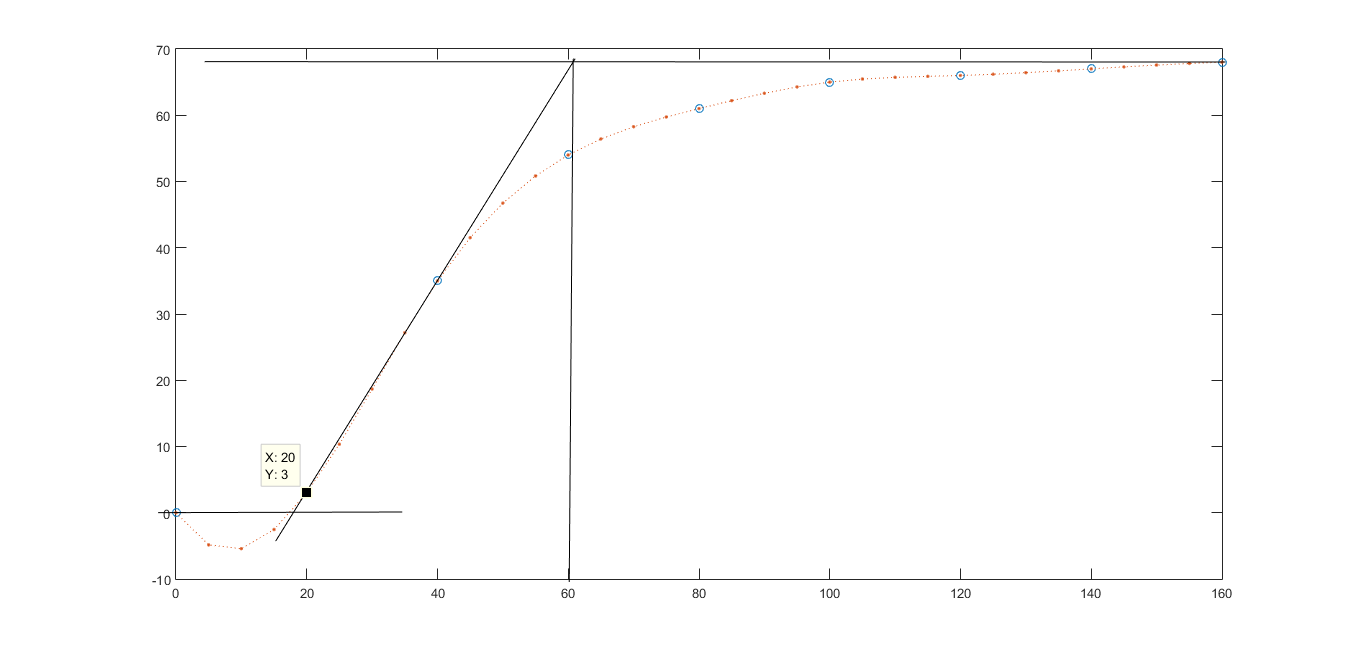
\includegraphics[width=0.9\textwidth]{03_Loesungskonzept/pictures/Sprungantwort.png}
\caption{Die Schrittantwort des DC-Motor im Matlab}
\label{fig:schrittantwort}
\end{figure}
Daraus konnten die Konstanten Tg=63ms und Tu=17ms ausgelesen werden(Einführung in die Regeltechnick S.71). Nach den Einstellregeln nach Chien-Hrones-Reswick konnten die Konstanten Tn, Tv und Kp berechnet werden(Einführung in die Regeltechnick S.215). Daraus ergaben sich die Werte Kp1=2.22, Tn=0.063, Tv=0.0085.
Diese Werte sind jedoch für kontinuierliche Regler und nicht wie in diesem Fall für diskrete Regler. Damit die Werte korrekt sind, mussten die Werte noch weiter verrechnet werden.(Einführung in die Regeltechnick S.247)
\[ T=Abtastperiodendauer=50ms\]
\[ Kp=Kp1*32=2.22*32=72\]
\[ Ki=Kp1*32*T/(2*Tn)=2.22*32*0.05/(2*0.063)=28\]
\[ Kd=Kp1*32*2*Tv/T=2.22*32*2*0.0085/0.05=5.44 =>5\]
Diese Werte sind die Regelparameter. Die Multiplikation mit 32 ergibt sich dem Grund, dass auf dem Mikrocontroller nicht mit Fließkommazahlen gerechnet wird. Somit werden die Werte bei den Parameter hochskaliert und später nach der Verrechnug mit der Regelabweichung wieder dividiert.
Diese Parameter wurden programmiert und ausgemessen. Ein Sollgeschwindigkeit von 150mm/s wurde dem Regler vorgegeben (entspricht einem Encoderwert von 108)
\begin{figure}[H]%Position festigen
\centering
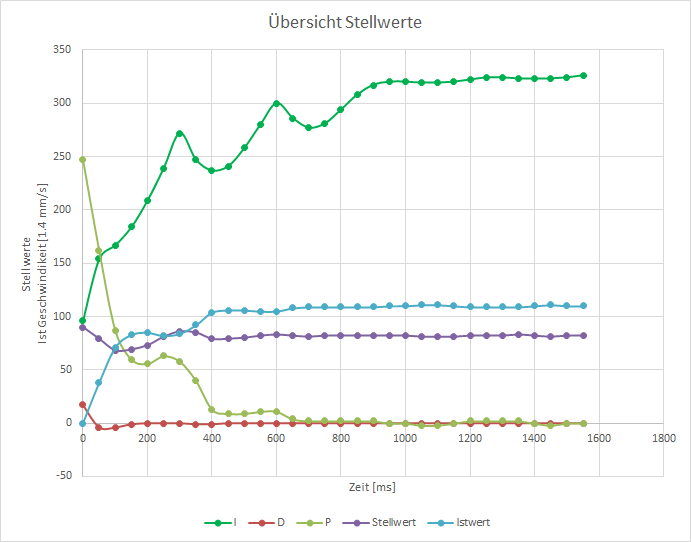
\includegraphics[width=0.9\textwidth]{03_Loesungskonzept/pictures/StellwertePID.png}
\caption{Die Istwert verglichen mit dem Stellwert}
\label{fig:IstSollwertVergleich}
\end{figure}
Hier zeigt sich, dass der Regler nicht Perfekt eingestellt ist, jedoch nach einer halben Sekunden den Sollwert erreicht hat. Dies ist für unsere Anwendung ausreichend und wurde deshalb so belassen.\\[0.2cm]
\textbf{Berechnung Encoder}\\[0.2cm]
Damit die Drehzahl des Motors ermittelt werden kann, braucht es einen Encoder. Dieser wurde mit dem Antriebsmotor mitgeliefert. Dies war sehr nützlich, da somit keine eigene aufwändige Lösung nötig war. Der Encoder muss mit 5V gespiesen werden. Als Ausgang hat der Encoder zwei Signale. Hier sind diese zu sehen:

Mit Hilfe dieser beiden Signalen gibt es 48 Ticks pro Umdrehung des Motors (ohne Übersetzung). Damit sind es 48Ticks/Umdrehung * 47 (Übersetzung) = 2'256 Ticks pro tatsächlicher Motorenumdrehung. Dies ergäbe eine Genauigkeit von 0.027mm/Tick bei unserem Fahrzeug. Dies ist sehr viel, darum wurde entschieden nur ein Signal auszuwerten. Damit ergibt sich eine Genauigkeit von 0.05mm/Tick. Dies ist immer noch sehr präzise.
Die Auswertung des Signales geschieht im Mikrocontroller. Das Encodersiganl wird über einen Spannungsteiler auf einen Pin des Freedomboard geführt. Diese löst bei jeder Flankenänderung einen Interrupt aus. Im Interrupt wird einfach einen Zähler hochgezählt. Dieser Zähler wird alle 40ms ausgelesen und wieder auf Null gesetzt. Der ausgelesene Wert ist der Ausgangswert des Encoders. Bei voller Geschwindigkeit beträgt dieser Wert Beispielsweise 140 und bei halber Geschwindigkeit 70.

%***************************
\subsubsection{Schnittstellen}